\section{Inductive learning of logical (task) rules}
In real life it may be hard to express the planning problem explicitly.

In partincular defining the precondition and the constraints of actions is challenging.

Looking at the classical Reinforcement Learning loop:
\begin{figure}[H]
    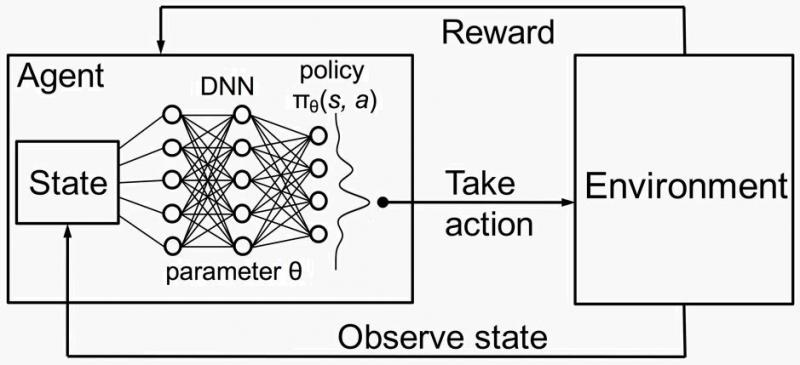
\includegraphics[width=0.5\textwidth]{img/RL.png}
    \centering
\end{figure}

RL is typically used to learn a state-action map (policy), given:
\begin{itemize}
    \item Transition model
    \item Reward model (hence goal)
    \item State and action spaces definition
    \item (possibly observation model under partial observability)
\end{itemize}

So in this context preconditions are logical representations of the policy mapping 
but Neural Networks are black box models.

However, we need explainable (or at least interpretable) models of agency in critical scenarios for trust and legal requirements.\\

When we execute the policy we know the state in which the agent is and the action taken by the agent.
One option could be to use Causal Discovery where State and action can be represented as time series so we want to find the causal relation between the state and the action.
The problem is that Causal Discovery outputs pairwise relations but those may not be expressive enough.

A more powerful approach would be to start from a logical formalization 
of the state and variables and then learn logical rules which can be used as a logical representation of the policy.
This task is usually known as \emph{Inductive logic programming}.

\subsection{Inductive logic programming}
Usually in Deductive Reasoning(what we've seen so far) we start from a Knowledge Base and we derive consequences of it.
In Inductive Reasoning we start from facts and we try to infer the logical rules which actually lead to that.

In Inductive logic programming we need to define:
\begin{itemize}
    \item \textbf{State-action pairs} (i.e examples) which may be Positive and Negatives
    \item \textbf{Background knowledge} which are known facts and axioms
    \item Set of possible rules(actions), or \textbf{search space}
\end{itemize}

The main definition of Inductive logic programming is Learning from entailment.
\begin{tcolorbox}[colback=red!5!white,colframe=red!75!black,title=\textbf{Definition 4: Learning from entailment}]
Consider a set of examples $E=\langle E^+,E^- \rangle$, where $E^+$ is a subset of positive examples and $E^-$ is a subset of negative examples.
The task of learning from entailment is defined as the tuple $T=\langle B, S_M, E \rangle$. THe goal of $T$ is to find $H\subseteq S_M$ such that:
\begin{itemize}
    \item $B\;\cup\;H\models E^+$
    \item $B\;\cup\;H\;\cup\;E^-\models \bot$
\end{itemize}
\end{tcolorbox}
This means that we want to learn $H$(called hypotesis) that supports our positive
examples (i.e if we add the hypotesis to the Background knowledge $B$ we can entail
the positive examples) and that does not support (is in contraddiction with) the negative
examples (i.e if we add together the negative hypotesis, the background knowledge and the
negative examples we reach a contraddiction).\\

To understand better let's go back to the classical robot changing room example:\\

\begin{minipage}[t]{0.2\textwidth}
    \begin{figure}[H]
        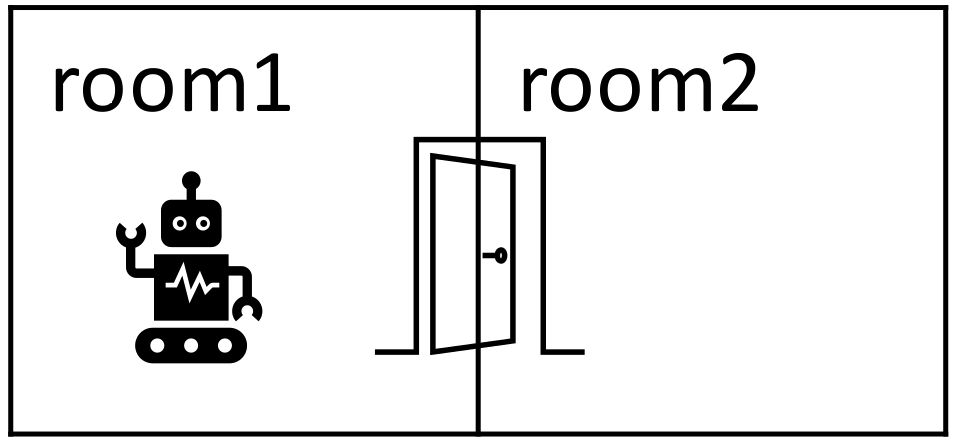
\includegraphics[width=\textwidth]{img/robot_room.png}
        \centering
    \end{figure}
\end{minipage}
\begin{minipage}[t]{0.8\textwidth}
    \begin{itemize}
        \item $E^+ = \{move(room1,room2,0), at(room1,0),
        not\;closed\_door(0), not\;closed\_door(1),
        at(room2,1)\}$
        \item $\{move(room2,room1,0)\}$
        \item $B = \{room(room1), room(room2), at(A,T) \leftarrow move(A,B,T-1), time(0..N)\}$
        \item $S_{M}=\{\\
                move(A,B,T) \leftarrow closed\_door(T); \\
                move(A,B,T) \leftarrow at(A,T);\\
                move(A,B,T) \leftarrow at(A,T), not\;closed\_door(T);\\
                \ldots\} \; \text{and all possible combinations}$
    \end{itemize}
\end{minipage}

\vspace{0pt}
If we apply learning from entailment here, we can learn the following hypotesis:\\
$H = \{move(A,B,T) \leftarrow at(A,T)\}\;\text{OR}\;\{move(A,B,T)\leftarrow at(A,T), not\;closed\_door(T)\}$.\\

Those are only some examples since multiple hypotheses can be found.
We are observing a limited number of task realizations we will never be sure to capture correct and complete knowledge!

\begin{tcolorbox}[colback=red!5!white,colframe=red!75!black,title=\textbf{Definition 5: Partial interpretation}]
Let $P$ be an ASP program. Any set of ground atoms that can be generated from axioms in $P$ is an interpretation of $P$.
Given an interpretation $I$ of $P$, a pair of subset of ground atoms $e=\langle e^{inc}, e^{exc}\rangle$ is said to be a partial
interpretation extended by interpretation $I$ if $e^{inc} \subseteq I$ and  $e^{exc} \cap I = \emptyset.$
\end{tcolorbox}

Given the previous definition an Answer Set can be sayed to be an interpretation since an Answer Set is definied as 
the minimal set of ground atoms which can be generated from the problem.
Also given the interpretation we can define also a partial interpretation which means a coupled subsets of ground atoms which we 
denote as the included set (\textcolor{Green}{$e^{inc}$}) and the excluded set (\textcolor{Red}{$e^{exc}$}) where the first is part
(i.e a subset) of the interpretation and the later has nothing in common with the Interpretation\\

If we start from an interpretation $I$:
\begin{equation*}
    I = AS = \{room(room1), room(room2), move(room1,room2,0), at(room1,0), at(room2,1), init(at(room2),1), \ldots\}
\end{equation*}
Some partial interpretation are:
\begin{align*}
    e1 &= \langle\textcolor{Green}{\{move(room1,room2,0), at(room1,0),at(room2,1)\}},\; \textcolor{Red}{\{move(room2,room1,0)\}}\rangle;\\
e2 &= \langle\textcolor{Green}{\{move(room1,room2,0), at(room1,0)\}},\;\textcolor{Red}{\{\}}\rangle
\end{align*}

Before we can move to learning Answer Set Programming we need to define other two definitions which are two substasks of learning from induction.
\begin{tcolorbox}[colback=red!5!white,colframe=red!75!black,title=\textbf{Definition 6: Brave Induction task}]
Let $\mathcal{T}=\langle B,S_M, E\rangle$, $H$, and $E=\langle E^+,E^- \rangle$ be as defined for learning from entailment 
under the AS semantics. Let $A$ be an answer set of the ASP program defined by $H \cup B$.
$\mathcal{T}$ is said to define a brave induction task if the goal set $H$ of hypotesis must satisfy:
\begin{equation*}
    \exists A\;s.t\;B \cup H \entails A: A\cap E^- =\emptyset\;\land\;E^+\subseteq A
\end{equation*}
\end{tcolorbox}

In this task we want to find an hypotesis which generates at least one answer set which excludes negative 
examples and entails positive examples.Positive examples should be entailed by \textbf{at least an answer set}
and Negative examples should be not entailed by \textbf{at least an answer set}.\\

The opposite of Brave Induction is the Cautious Induction:
\begin{tcolorbox}[colback=red!5!white,colframe=red!75!black,title=\textbf{Definition 7: Cautious induction task}]
    Let $\mathcal{T}=\langle B,S_M, E\rangle$, $H$, and $E=\langle E^+,E^- \rangle$ be as defined for learning from entailment 
    under the AS semantics. Let $A$ be an answer set of the ASP program defined by $H \cup B$.
    $\mathcal{T}$ is said to define a cautious induction task if the goal set $H$ of hypotesis must satisfy:
    \begin{equation*}
        \forall A\;s.t\;B \cup H \entails A: A\cap E^- =\emptyset\;\land\;E^+\subseteq A
    \end{equation*}
\end{tcolorbox}

Contrary to the brave induction Positive examples should be entailed by \textbf{all answer sets} and Negative examples should be not entailed by
\textbf{any answer set}

\subsection{Inductive learning of answer set programs (ILASP)}
Given the previous definitions we can give the definion of Inductive learning of answer set programs which is a particular specialization
of Learning from Entailment task.

\begin{tcolorbox}[colback=red!5!white,colframe=red!75!black,title=\textbf{Definition}]
The ILASP learning task $\mathcal{T}=\langle B,S_M, E\rangle$ is a tuple of background knowledge $B$, search space $S_M$ and examples $E=\langle E^+,E^- \rangle$ 
such that $E^+ (E^-)$ is the subset of positive (negative) examples. The goal of $\mathcal{T}$ is to find $H \subseteq S_M$ such that $\forall e\in E$, $e$ is a 
particular interpretation of the ASP program $B\cup H$. If AS is an answer set of the ASP program $H\cup B$ the following must hold:
\begin{align*}
    \forall e \in E^+\exists AS\;s.t\; B\cup H\entails AS: e \;\text{is extended by AS}\\
    \forall e \in E^-\cancel{\exists} AS\;s.t\; B\cup H\entails AS: e \;\text{is extended by AS}
\end{align*}
\end{tcolorbox}

The ILASP task is a combination of brave and cautious tasks. 
The goal of ILASP task is to find an hypotesis which satisfies this two conditions:
\begin{itemize}
    \item Positive examples should be entailed by \textbf{at least an answer set} (brave)
    \item Negative examples should be not entailed \textbf{by any answer set} (cautious)
\end{itemize}
In this task examples are structured as partial interpretations.\\

For the sake of this course we are particularly interested in ILASP under CDPIs (context-dependent partial interpretations).
\begin{tcolorbox}[colback=red!5!white,colframe=red!75!black,title=\textbf{Definition 3: Context-dependent partial interpretation (CDPI)}]
A CDPI of an ASP program $P$ with an interpretation $I$ is a tuple $e_c=\langle e, C\rangle = \langle e^{inc},e^{exc}, C\rangle$, where $e$ is a partial interpretation, and $C$ is an 
ASP program called $context$. $I$ is said to extend $e_c$ if $e^{inc}\cup C\subseteq I$ and $(e^{exc}\cup C) \cap I = \emptyset$
\end{tcolorbox}

\begin{tcolorbox}[colback=red!5!white,colframe=red!75!black,title=\textbf{Definition 4: ILASP task with CDPIs}]
An ILASP learning task with CDPIs is a tuple $\mathcal{T}=\langle B,S_M, E\rangle$, where $E=\langle E^+,E^- \rangle$ is a set of CDPIs
with context $C$. We say that $H\subseteq S_M$ is a solution to $\mathcal{T}$ if the following hold:
\begin{align*}
    \forall e \in E^+\exists AS\;s.t\; B\cup H\cup C\entails AS: e \;\text{is extended by AS}\\
    \forall e \in E^-\cancel{\exists} AS\;s.t\; B\cup H\cup C\entails AS: e \;\text{is extended by AS}
\end{align*}
\end{tcolorbox}

To understand better let's go back to our usual example:\\

\begin{minipage}[t]{0.2\textwidth}
    \begin{figure}[H]
        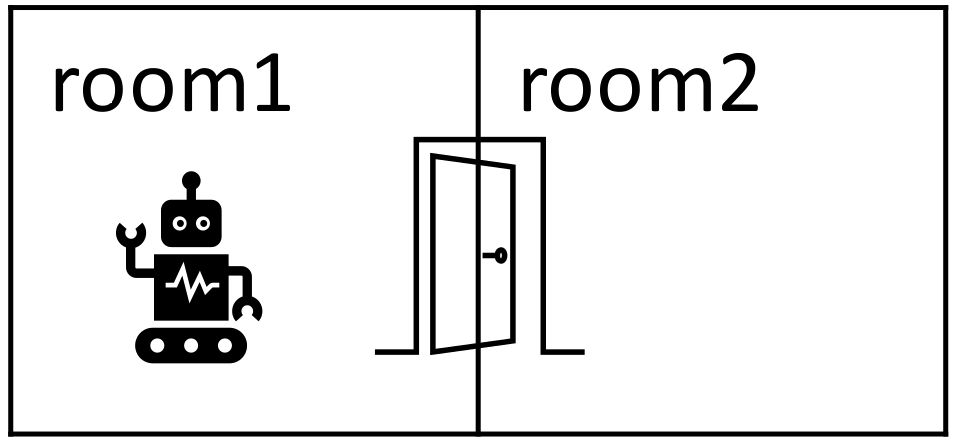
\includegraphics[width=\textwidth]{img/robot_room.png}
        \centering
    \end{figure}
\end{minipage}
\begin{minipage}[t]{0.8\textwidth}
    \begin{itemize}
        \item $\textcolor{Blue}{e^{inc}},\textcolor{Green}{e^{exc}},\textcolor{Red}{C}$
        \item $E^+ = \langle\{\textcolor{Blue}{move(room1,room2,0)}\},\textcolor{Green}{\{\}}, \{\textcolor{Red}{at(room1,0),at(room2,1)}\}\rangle$
        \item $E^- = \langle\{\textcolor{Blue}{move(room2,room1,0)}\},\textcolor{Green}{\{\}}, \{\textcolor{Red}{at(room1,0),at(room2,1)}\}\rangle$
        \item $B = \{room(room1), room(room2), at(A,T) :-\; move(A,B,T-1), time(0..N)\}$
        \item $S_{M}=\{\\
                    move(A,B,T) :-\; closed\_door(T), room(A), room(B). \\
                    move(A,B,T) :-\; at(A,T), room(B).\\
                    \text{:-}\; move(A,B,T), closed\_door(T).\\
                    \ldots\} \;$
    \end{itemize}
\end{minipage}

We still have positive and negative examples but we split our observations into Excluded and Included sets.
Particularly actions are placed into the included set and the rest of the atoms into the context.
Similarly for the negative examples we have that the included set contains not executed actions  and the rest of the atoms into the context.

This is done because in ILASP we want to discover action preconditions.
Doing so we have that actions(possible heads of hypothesis) and the context (possible body) are separated.\\

A possible hypotesis which satisfies the ILASP task condition is:
\begin{equation*}
    H = \{move(A,B,T) :- at(A,T), room(B).\}
\end{equation*}

Until now we've had an empty excluded set, so why do we need it?

Assume we don't have negative examples but I add something to the excluded set in the positive example:
\begin{itemize}
    \item $E^+ = \{\{move(room1,room2,0)\},\{\textbf{move(room2,room1,0)}\}, \{at(room1,0),at(room2,1)\}\}$
    \item $E^- = \langle\{\},\{\},\{\}\rangle$
    \item $B = \{room(room1), room(room2), at(A,T) :-\; move(A,B,T-1), time(0..N)\}$
    \item $S_{M}=\{\\
                move(A,B,T) :-\; closed\_door(T), room(A), room(B). \\
                move(A,B,T) :-\; at(A,T), room(b).\\
                move(A,B,T) :-\; at(A,T), closed\_door(T);\\
                \ldots\} \;$
\end{itemize}
In this case the Hypotesis will be the same as before.\\

Now lets consider the three romms environment:

\begin{minipage}[t]{0.2\textwidth}
\begin{figure}[H]
    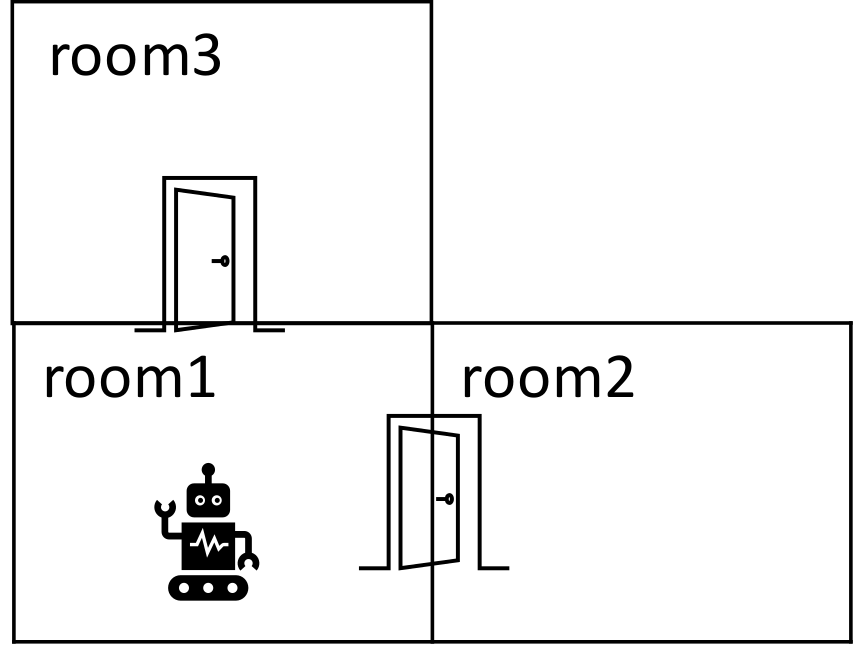
\includegraphics[width=0.9\textwidth]{img/three_room.png}
    \centering
\end{figure}

\end{minipage}
\begin{minipage}[t]{0.8\textwidth}
    $room(room1;room2).\\
    at(room1,0).\\
    closed\_door(0).\\
    0\;\{move(A,B,T) : at(A,T), room(B)\}\;1.\\
    init(at(A),T) \text{:-}\; move(B,A,T-1).\\
    term(at(A),T) \text{:-}\; move(A,B,T-1), A!=B.\\
    at(A,T) \text{:-}\; init(at(A),T).\\
    at(A,T) \text{:-}\; at(A,T-1), not\;term(at(A),T).\\
    \text{:-}\; move(A,B,T), closed\_door(T).\\
    \text{:-}\; not\;at(room2,1), not\;at(room3,1).\\
    AS1 = \{room(room1), room(room2), \ldots, move(room1,room2,0)\}\\
    AS2 = \{room(room1), room(room2), \ldots, move(room1,room3,0)\}$
\end{minipage}\\

If we formalize this into a ILASP task:
\begin{itemize}
    \item $E^+ = \{\{move(room1,room2,0)\},\{\textbf{move(room1,room3,0)}\}, \{at(room1,0),at(room2,1)\}\}$
    \item $E^- = \langle\{\},\{\},\{\}\rangle$
    \item $B = \{room(room1), room(room2), at(A,T) :-\; move(A,B,T-1), time(0..N)\}$
    \item $S_{M}=\{\\
                move(A,B,T) :-\; closed\_door(T), room(A), room(B). \\
                move(A,B,T) :-\; at(A,T), room(B).\\
                \text{:-}\; move(A,B,T), closed\_door(T).\\
                0\;\{move(A,B,T) : at(A,T), room(B)\}\;1\\
                \ldots\} \;$
\end{itemize}
we can learn two hypotesis:
\begin{itemize}
    \item $H = \{move(A,B,T) :- at(A,T), room(B).\}$
    \item $H = \{0\; \{move(A,B,T) : at(A,T), room(B).\}\; 1\}$
\end{itemize}

If we remove the excluded set and add again the negative example:
\begin{itemize}
    \item $E^+ = \{\{move(room1,room2,0)\},\{\}, \{at(room1,0),at(room2,1)\}\}$
    \item $E^- = \langle\{\textbf{move(room1,room3,0)}\},\{\},\{at(room1,0),at(room2,1)\}\rangle$
    \item $B = \{room(room1), room(room2), at(A,T) :-\; move(A,B,T-1), time(0..N)\}$
    \item $S_{M}=\{\\
                move(A,B,T) :-\; closed\_door(T), room(A), room(B). \\
                move(A,B,T) :-\; at(A,T), room(B).\\
                \text{:-}\; move(A,B,T), closed\_door(T).\\
                0\;\{move(A,B,T) : at(A,T), room(B)\}\;1\\
                \ldots\} \;$
\end{itemize}
We have that the second hypotesis is no longer valid:
\begin{itemize}
    \item $H = \{move(A,B,T) \text{:-} at(A,T), room(B).\}$
    \item\st{$H = \{0\; \{move(A,B,T) : at(A,T), room(B).\}\; 1\}$}
\end{itemize}
Because there must be no answer set which extends the negative example.
So the differnce between Negative examples and excluded set stands in the 
different learning task which ilasp performs for positive and negative examples:
\begin{itemize}
    \item Positive examples $\rightarrow$ Brave Induction
    \item Negative examples $\rightarrow$ Cautious Induction
\end{itemize}

Usually what we do when creating an ILASP task is placing the observations in 
the positive examples and use the negative examples only when we want to enforce some safety constraints.\\

Going back to the Reinforcement Learning setting we stated at the beggining,
in this setting we know only about the observations we get and so Negative examples cannot be easily built.

\subsection{ILASP in practice}
